\documentclass[11pt]{article}

\usepackage[margin=1in]{geometry}
\usepackage[T1]{fontenc}
\usepackage[utf8]{inputenc}
\usepackage{lmodern}
\usepackage{setspace}
\usepackage{graphicx}
\usepackage{booktabs}
\usepackage{array}
\usepackage{amsmath}
\usepackage{amssymb}
\usepackage{hyperref}
\usepackage{xcolor}
\usepackage{lineno}

\hypersetup{
  colorlinks=true,
  linkcolor=blue,
  citecolor=blue,
  urlcolor=blue
}

\newcommand{\todoitem}[1]{\textcolor{red}{\textbf{[TODO: #1]}}}

\title{Humanoid Agent for Organoid Intelligence}

\author{
Rongzhou Chen \and Zhenyu Wu \and Shaohua Ma
}

\date{March 2, 2026}

\begin{document}
\maketitle
\linenumbers
\doublespacing

\begin{abstract}
Organoid experiments increasingly generate large, heterogeneous collections of brightfield images, tabular readouts, and single-cell analysis files, yet many groups still rely on fragmented scripts or manual inspection for quality control and early phenotyping. We present OrganoidAgent, an agent-orchestrated software system for organizing, previewing, and analyzing multimodal organoid datasets in a reproducible workflow. OrganoidAgent combines a lightweight Tornado backend with a progressive web interface and task-specific analysis modules for tabular data preview, archive introspection, TIFF rendering, and single-cell \texttt{.h5ad} summarization with automated two-dimensional embedding visualization. The system exposes standardized APIs for dataset listing, category-based filtering, preview generation, and archive extraction, enabling rapid triage of experimental outcomes before deeper modeling. We describe the architecture, implementation, and an evaluation protocol designed for translational organoid workflows, including quality control gates and pathway-specific analysis entry points. This manuscript provides a submission-ready technical foundation for a Nature-family methods paper and includes generated illustrative figures plus explicit placeholders for experiment-specific quantitative benchmarking, biological validation, and ablation analyses.
\end{abstract}

\section*{Main}

\section{Introduction}
Organoid models are increasingly used to study tissue development, disease mechanisms, and therapeutic response under physiologically relevant conditions. In practice, organoid studies produce multimodal artifacts at different scales: microscopy image stacks, compressed archives, tabular summaries, and single-cell feature matrices. Despite growing data volume, routine analysis pipelines remain labor-intensive and often brittle, with limited standardization across experiments.

Agent-oriented systems can improve this bottleneck when they are used as orchestration layers over explicit, auditable computational tools rather than opaque black-box decision makers. We therefore designed OrganoidAgent as a practical platform to streamline data intake, dataset browsing, preview generation, and first-pass computational phenotyping for organoid experiments.

The core goals were: (i) reduce time from raw data acquisition to interpretable previews, (ii) provide a uniform API surface across heterogeneous file types, (iii) support reproducible quality-control and analysis handoff, and (iv) maintain low operational complexity for laboratory deployment.

\section{System Overview}
OrganoidAgent is implemented as a Python backend (Tornado) with a progressive web application frontend. The backend exposes HTTP endpoints for dataset-level and file-level operations, while the frontend enables rapid interactive exploration. The system is organized around five core capabilities:

\begin{enumerate}
\item \textbf{Dataset inventory and file indexing.} Recursive scanning of dataset folders with file count and storage summaries.
\item \textbf{Type-aware preview generation.} Automatic handling of tables (CSV/TSV/Excel), analysis files (H5AD/HDF5), images (including TIFF), archives (ZIP/TAR/TGZ), and compressed text (GZ).
\item \textbf{Single-cell analysis preview.} Fast summary extraction from \texttt{.h5ad} files (observations, variables, metadata keys) with embedding-based scatter previews (UMAP/t-SNE/PCA when available; sampled PCA fallback otherwise).
\item \textbf{Archive introspection and extraction.} Entry listing with optional first-image preview and API-driven extraction into tracked subfolders.
\item \textbf{Category routing for analysis stages.} API filters to group files into dataset, segmentation, feature, and analysis categories for downstream workflows.
\end{enumerate}

\section{Implementation Details}
\subsection{Backend architecture}
The backend is centered on deterministic, stateless API handlers that wrap utility functions for file classification, safe path resolution, and preview rendering. A strict path sanitizer ensures requests remain inside the configured dataset root. Preview artifacts are cached using hash-derived filenames in a dedicated cache directory, minimizing repeated compute and improving responsiveness for interactive use.

\subsection{Analysis-specific preview methods}
For table files, OrganoidAgent returns bounded row previews and column metadata. For TIFF microscopy files, a representative frame is selected and normalized for visualization, with size-constrained thumbnails generated for browser display. For single-cell \texttt{.h5ad} files, the backend attempts to reuse available embeddings from \texttt{obsm}; if absent, it computes a sampled PCA preview to provide a fast structural summary. These previews are intended for triage and exploratory QA, not for final inferential reporting.

\subsection{Frontend interaction model}
The web interface consumes the backend APIs to support dataset browsing, file inspection, and type-specific previews from a unified surface. This design allows wet-lab and computational users to align on the same intermediate artifacts before formal statistical analysis.

\section{Evaluation Framework for Biological Studies}
To support publication-grade validation, we define an evaluation framework that separates engineering reliability from biological performance:

\begin{enumerate}
\item \textbf{Operational reliability.} API success rate, median preview latency by file type, cache hit ratio, and extraction completion rate.
\item \textbf{Data quality and triage utility.} Fraction of files receiving interpretable previews, error taxonomy, and manual agreement on preview correctness.
\item \textbf{Biological analysis readiness.} Agreement between rapid previews and full offline pipelines on key endpoints (for example, dimensional structure in single-cell datasets).
\item \textbf{Workflow impact.} Reduction in analyst time-to-first-insight relative to ad hoc script-based workflows.
\end{enumerate}

\noindent
\todoitem{Insert quantitative benchmarking results on internal datasets, with confidence intervals and replicate definitions.}

\subsection{Quantitative formulation}
We define the primary computational objectives explicitly to support reproducibility and ablation studies.

\paragraph{Quality control score.}
For frame $i$, a normalized quality score is defined as
\begin{equation}
Q_i = w_f \hat{f}_i + w_c \hat{c}_i + w_a (1-\hat{a}_i),
\end{equation}
where $\hat{f}_i$ is normalized focus sharpness, $\hat{c}_i$ is normalized illumination consistency, $\hat{a}_i$ is artifact burden, and $w_f + w_c + w_a = 1$.

\paragraph{Segmentation accuracy.}
Given prediction mask $M$ and reference mask $G$, the Dice coefficient is
\begin{equation}
\mathrm{Dice}(M,G)=\frac{2|M\cap G|}{|M|+|G|},
\end{equation}
and the mean boundary distance is
\begin{equation}
E_b=\frac{1}{|\partial G|}\sum_{p\in\partial G}\min_{q\in\partial M}\lVert p-q\rVert_2.
\end{equation}

\paragraph{Tracking association cost.}
For a detection $j$ at time $t+1$ and track hypothesis $k$, the assignment cost is
\begin{equation}
C_{jk}= \alpha \lVert x_j^{t+1}-\hat{x}_k^{t+1}\rVert_2 + \beta \left(1-\mathrm{IoU}(b_j,b_k)\right),
\end{equation}
where $\hat{x}_k^{t+1}$ is Kalman-predicted location and $\mathrm{IoU}(b_j,b_k)$ measures box overlap.

\paragraph{Infiltration phenotype score.}
With inward and outward boundary crossings $N_{\text{in}}(t)$ and $N_{\text{out}}(t)$, we define
\begin{equation}
I=\frac{1}{T}\sum_{t=1}^{T}\frac{N_{\text{in}}(t)-N_{\text{out}}(t)}{\max(1,N_{\text{tot}}(t))}.
\end{equation}

\paragraph{Growth forecasting objective.}
For early trajectory features $z_{1:\tau}$ and late endpoint $y_T$, the predictor is
\begin{equation}
\hat{y}_T=f_{\theta}(z_{1:\tau}),
\end{equation}
optimized by
\begin{equation}
\mathcal{L}(\theta)=\frac{1}{N}\sum_{n=1}^{N}\left(y_T^{(n)}-\hat{y}_T^{(n)}\right)^2+\lambda\lVert\theta\rVert_2^2.
\end{equation}

\section{Representative Use Cases}
\subsection{Multimodal dataset triage}
A common entry point is a mixed dataset containing microscopy files, archive bundles, and analysis matrices. OrganoidAgent enables rapid identification of actionable files by category, immediate visual checks on image quality, and lightweight statistical context for single-cell objects.

\subsection{Segmentation and feature-engineering handoff}
Category-specific API routes separate candidate segmentation inputs (image/archive) from feature tables and analysis matrices, supporting modular downstream pipelines while maintaining traceability to original data assets.

\subsection{Archive-first ingestion}
When data arrive as compressed bundles, OrganoidAgent can inspect archive contents, preview representative image entries, and extract files into deterministic locations to simplify reproducible preprocessing.

\section{Generated Figures}
\begin{figure}[t]
\centering
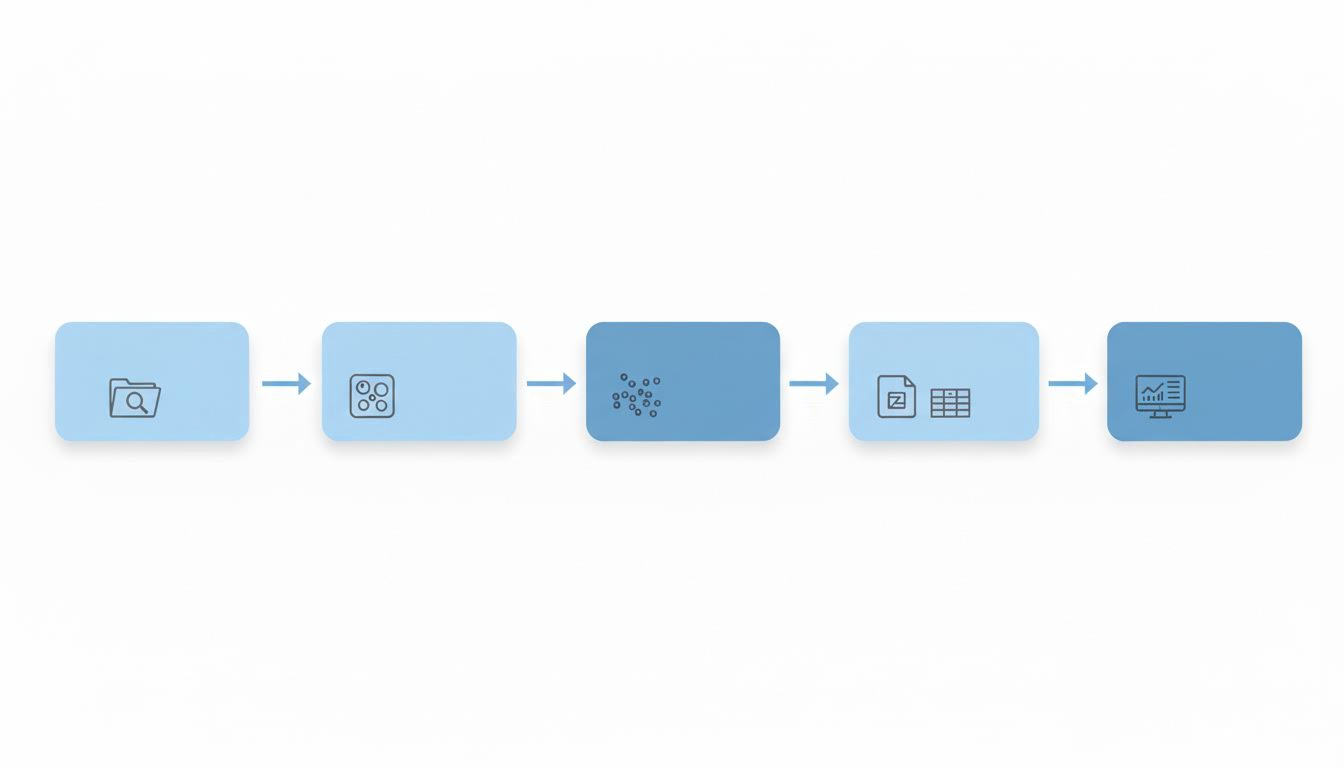
\includegraphics[width=\linewidth]{figures/001_fig1_architecture_organoidagent_architecture.png}
\caption{Generated system architecture figure. The panel illustrates an end-to-end OrganoidAgent workflow from multimodal dataset intake to API-driven preview generation and interactive reporting.}
\label{fig:architecture_generated}
\end{figure}

\begin{figure}[t]
\centering
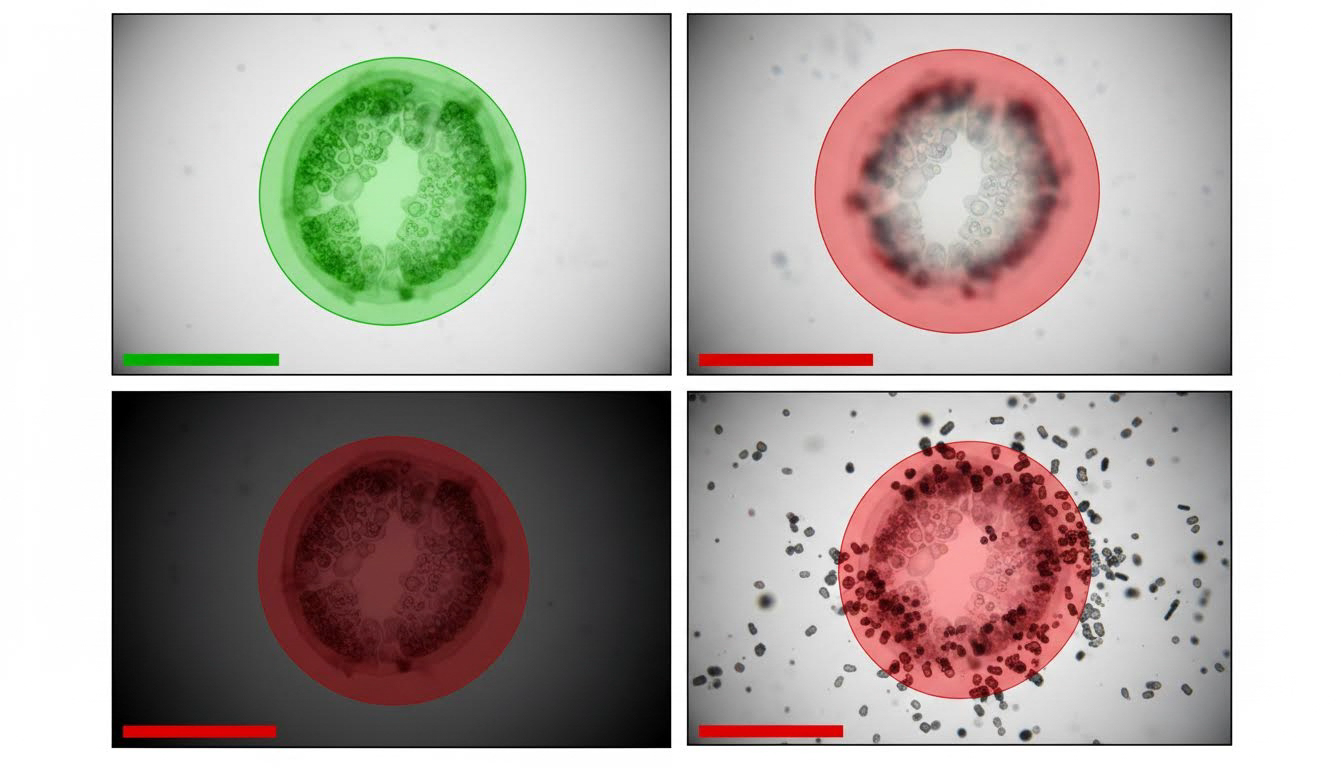
\includegraphics[width=\linewidth]{figures/002_fig2_qc_quality_control_examples.png}
\caption{Generated quality-control examples panel for brightfield organoid imaging, showing representative quality regimes and artifact patterns used for triage.}
\label{fig:qc_generated}
\end{figure}

\begin{figure}[t]
\centering
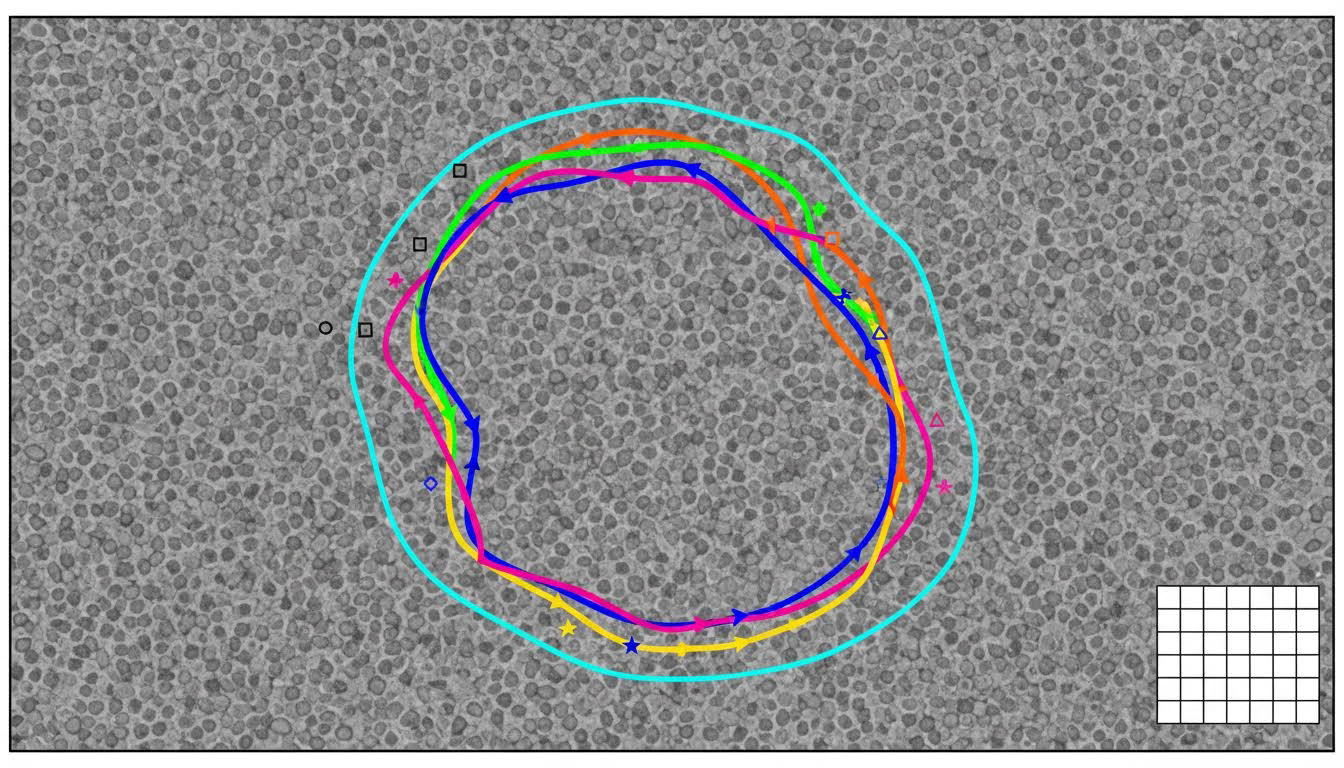
\includegraphics[width=\linewidth]{figures/003_fig3_segtrack_segmentation_tracking_overlay.png}
\caption{Generated segmentation and tracking visualization panel with organoid boundary overlays and immune-cell trajectory patterns.}
\label{fig:segtrack_generated}
\end{figure}

\begin{figure}[t]
\centering
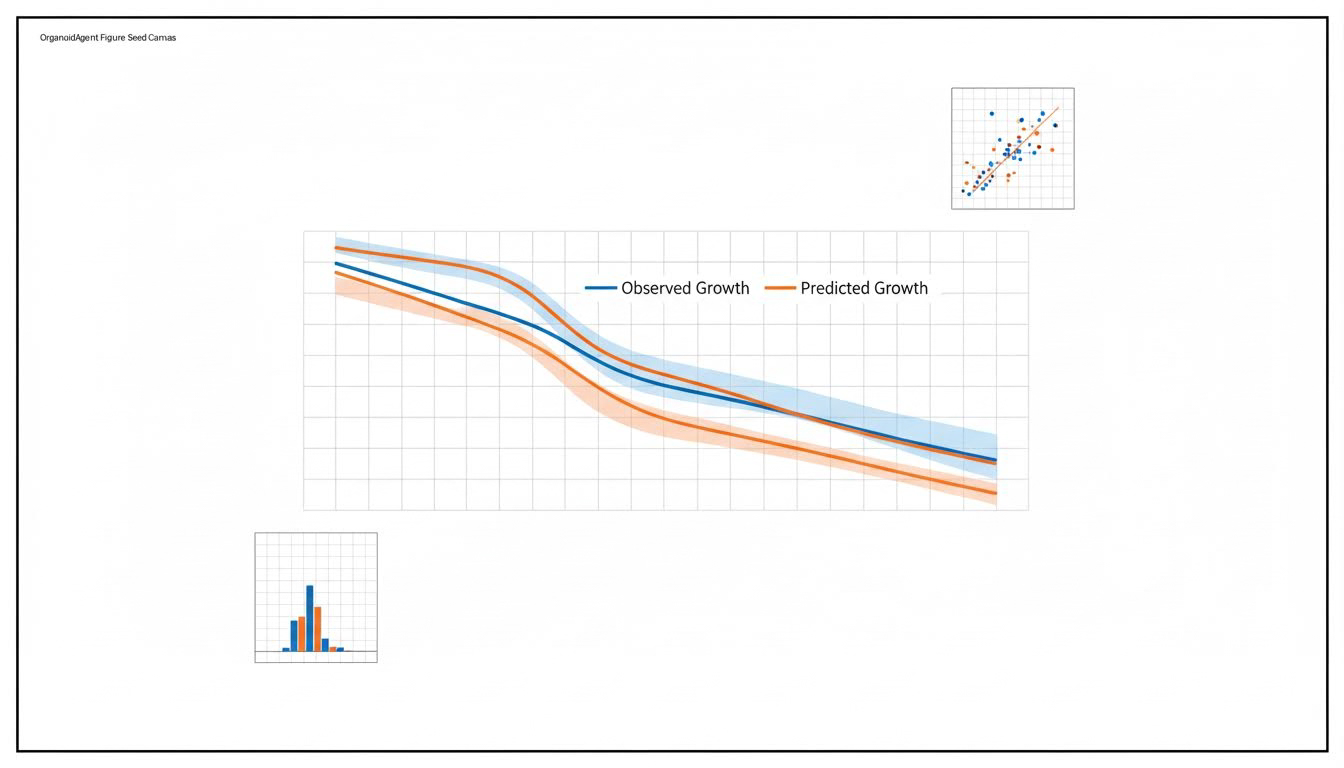
\includegraphics[width=\linewidth]{figures/004_fig4_forecast_growth_forecasting_curve.png}
\caption{Generated growth-forecasting panel depicting predicted-versus-observed trend behavior and uncertainty structure.}
\label{fig:forecast_generated}
\end{figure}

\section{Discussion}
OrganoidAgent addresses a practical and under-served stage of organoid analysis: rapid, reproducible conversion of heterogeneous raw files into inspectable computational artifacts. The current implementation prioritizes robust file handling, preview generation, and workflow orchestration. This foundation is compatible with future integration of segmentation, cell tracking, phenotyping, and predictive modeling modules.

The framework also clarifies the role of agentic systems in biomedical data science. Rather than replacing domain expertise, the agent layer standardizes routine operations, surfaces quality signals early, and creates a consistent interface between experimental and computational teams.

Key limitations include dependence on local file organization conventions, variable metadata quality across studies, and the need for study-specific validation before inferential claims. For Nature-family publication standards, future versions should include controlled ablations, cross-batch generalization tests, and prospective biological endpoint validation.

\section{Methods}
\subsection{Software environment}
OrganoidAgent is implemented in Python with Tornado for web serving. Optional dependencies include pandas (table preview), anndata plus numpy (single-cell preview), Pillow (image rendering), and tifffile (TIFF handling). The application can be run locally on standard laboratory workstations.

\subsection{File typing and routing}
File classification uses extension-based routing with explicit support for image, table, analysis, archive, compressed-text, and document types. Unsupported files remain accessible via direct download.

\subsection{Preview generation}
Table previews are row-limited for responsiveness. TIFF previews use frame normalization to map intensity ranges for browser display. Single-cell previews extract metadata dimensions and attempt embedding reuse before fallback PCA with random subsampling.

\subsection{Security and data locality}
The backend uses sanitized relative paths and resolves all requests under the dataset root to prevent path traversal. All processing is local to the deployment environment.

\section{Data Availability}
The data used to generate publication figures and benchmark tables should be deposited in a public repository at the time of submission.
\todoitem{Insert accession IDs and persistent links.}

\section{Code Availability}
OrganoidAgent source code is available in the project repository.
\todoitem{Insert public repository URL and tagged release hash used for the manuscript.}

\section{Acknowledgements}
We thank collaborators and laboratory members for discussions on organoid workflow requirements and evaluation priorities.
\todoitem{Insert funding sources and grant numbers.}

\section{Author Contributions}
R.C., Z.W., and S.M. conceptualized the study. R.C. and Z.W. implemented the software and performed computational analysis. S.M. supervised the project. All authors contributed to manuscript writing and revision.

\section{Competing Interests}
The authors declare no competing interests.

\begin{thebibliography}{10}

\bibitem{huch2017}
Huch, M. \& Koo, B.-K. Modeling mouse and human development using organoid cultures. \textit{Development} \textbf{142}, 3113--3125 (2015).

\bibitem{fatehullah2016}
Fatehullah, A., Tan, S. H. \& Barker, N. Organoids as an in vitro model of human development and disease. \textit{Nat. Cell Biol.} \textbf{18}, 246--254 (2016).

\bibitem{wolf2018scanpy}
Wolf, F. A., Angerer, P. \& Theis, F. J. SCANPY: large-scale single-cell gene expression data analysis. \textit{Genome Biol.} \textbf{19}, 15 (2018).

\bibitem{tornadoweb}
FriendFeed. Tornado Web Server and Tools.
\url{https://www.tornadoweb.org/} (accessed March 2, 2026).

\bibitem{anndata}
Virshup, I. \textit{et al.} The anndata ecosystem for annotated data matrices.
\url{https://anndata.readthedocs.io/} (accessed March 2, 2026).

\bibitem{cellpose}
Stringer, C. \textit{et al.} Cellpose: a generalist algorithm for cellular segmentation. \textit{Nat. Methods} \textbf{18}, 100--106 (2021).

\end{thebibliography}

\end{document}
